\setchapterpreamble[u]{\margintoc}
\chapter{Transition Scenarios}
\labch{transition_scenarios}

We will assume four main categories of transition scenarios for each country as a first-order approximation.

\begin{itemize}
	\item \textbf{S1:} 100\% single renewable technology scenarios
	\item \textbf{S2:} 100\% multiple renewable technologies scenarios
	\item \textbf{S3:} 100\% Nuclear scenarios
	\item \textbf{S4:} Mix of nuclear with multiple renewable technologies scenarios
\end{itemize}

The Nuclear Scenario replaces and expands the nuclear program in the countries where it exists to cover 100\% of the electrical demand, and create one where it does not. The 100\% single renewable scenario phases out both fossil fuels and nuclear energy from the electricity and energy generation mix, and replaces them with one technology\sidenote[][-2mm]{Only onshore wind power, or only solar power, for example}. Of course, those scenarios are an exaggeration of what the near future may look like, but it will still be interesting to compare their respective viability. No scenarios involving fossil fuels for electricity generation are acceptable, as the end goal is to transition to low carbon energy sources. The 100\% multiple renewable scenario takes this a step further by allowing the renewable mix to be accounted for. And finally, we show what the impact of a mix of nuclear and renewable could look like.

We will not consider exports or imports of electricity, as we assume that the neighbors encounter similar issues in their transitions, and energy independence is considered an important factor. Note that this assumption is valid when considering the first order impact of our scenarios. Geopolitics make it so that full cooperation with high dependence for something as critical as the energy infrastructure is not something nations will accept readily, even between strong allies.


Again, recall that we want only a simplistic first-order comparison. Our goal is not to build a complex model, optimized and tuned to decades of historical and projected data\sidenote[][-2mm]{Those models are set in an ideal Utopian world where crisis are non-existent and society is more stable than any other time in history. I am rooting for this, but I like to stay reasonable}. We aim to show what one can reasonably expect from various scenarios and draw conclusions from this. Policies have never been made on complex, perfectly optimized simulations. If the first order calculation does not agree with a complex model, it does not mean the complex model is wrong per se, but that its implementation is unlikely to work as intended, because humans are not always rational actors unfortunately.

Finally, we have discussed this previously: we want a sustainable grid, looking at a first-order optimal solution at a horizon of 100 years.

\section{Scenarios S1}

We define the S1 scenarios as being the 100\% single renewable energy scenarios. This implies that for each scenario in this category, the entire energy generation fleet is driven by one technology. This is of course an implausible assumption, but one that will allow us to derive useful information nonetheless.

\begin{kaobox}[frametitle=S1 scenarios]
\begin{itemize}
	\item \textbf{S1a:} 100\% Wind (onshore) coupled with Pumped Hydroelectric Storage
	\item \textbf{S1b:} 100\% Wind (onshore) coupled with Batteries Storage
	\item \textbf{S1c:} 100\% Wind (offshore) coupled with Pumped Hydroelectric Storage
	\item \textbf{S1d:} 100\% Wind (offshore) coupled with Batteries Storage
	\item \textbf{S1e:} 100\% Solar coupled with Pumped Hydroelectric Storage
	\item \textbf{S1f:} 100\% Solar coupled with Batteries Storage scenarios
\end{itemize}
\end{kaobox}

By its nature, a grid composed of 100\% renewable resources is not viable to deliver a society similar to what we are all used to currently, and what I'm fairly certain we all wish for the future\sidenote[][-2mm]{This does not mean no consumption adaptation, it simply means we are looking to lower the bar of necessary changes to let it be realistic}. We will use the two most prevalent technologies in the discussions, pumped hydroelectricity storage and batteries. So, exactly how much storage do we need?

To answer this question, the first thing we need to know is:

\begin{itemize}
\item What is the maximum period of time where our needs could be unmet?
\end{itemize}

An important thing to note here is that when we say that the needs are not meet, it does not mean that we get no power from our installed capacity. It means that we do not get enough power from our installed capacity. Ten days of wind production at 20\% is equivalent to two days of no wind at all.

Common scenarios are a gloomy week, or a sustained storm. In those cases, solar and wind production will be hampered. It is not unreasonable, and pretty accepted, to think that 7 days of storage would be needed. Keep in mind that if you do not have enough storage in place and run out, the whole economy stops. We will modify the duration to test the sensitivity to storage need, from 1 to 7 days.


\begin{remark}
The energy to store is given by~\ref{energy_store}, $t$ varying between 1 and 7 days (it has to be given in number of hours).

\begin{equation}\label{energy_store}
E_s = t * \frac{E_a}{8760}
\end{equation}

\end{remark}

Round-trip efficiency represent the fraction of the electricity that you put in that you can expect to get back. Indeed, you will not get back everything you sent to your storage, due to cable losses, inverter or mechanical losses, and various other factors. This efficiency is variable between technologies and over time. A good approximation is between 65\% and 85\%\sidenote[][-2mm]{As an example, for pumped storage, the main sources of losses are approximately 5\% to the network itself, 80\% to the pumping stations and 85\% to the turbines, which translates to 65\%, and thus a loss to storage of 35\%.}. 

This has a strong implications. In order to get back the energy you would need, you have to send $\frac{1}{0.85} = 1.18$ to $\frac{1}{0.65} = 1.55$ times as much electricity. This has a potential impact on the capacity that has to be installed to begin with.

We will assume that this does not matter for our first order calculation, and that we have enough power generation to fill in sufficient storage power capacity by default. Additionally, we consider that the extra power generated when demand is low can be easily curtailed or used in alternate, non-time sensitive process. This encompasses hydrogen production or desalination, for example, two energy intensive processes\sidenote[][-2mm]{Energy is only one of the drivers of these processes challenges.}.

All the scenarios discussed will consider the existing grid, decommission what needs to be decommissioned, and rebuild everything from scratch to a 100\% technology penetration for a period of 100 years.

For simplicity sake, we do not consider the currently installed capacity of the given production technology. This does not impact the results, given the scale and timeframe of the transitions.


\section{Scenarios S2}

Obviously, the one-generating-technology scenarios are on the extreme, unrealistic side. The load factor considered in a renewable mix will be more advantageous due to a combination effect\sidenote[][-2mm]{You can have wind when you do not have solar, and vice versa. But keep in mind that the limiting factor will often be windless or low-wind nights, which are not uncommon, and which you need to plan for with storage}.

In those scenarios, we will play with the type of renewable mix we develop during the transition, by changing the ratio of solar versus wind power notably.


\begin{kaobox}[frametitle=S2 scenarios]
\begin{itemize}
	\item \textbf{S2a:} 50\% Wind (75\% onshore and 25\% offshore), 50\% Solar, coupled with pumped hydroelectric storage
	\item \textbf{S2b:} 50\% Wind (75\% onshore and 25\% offshore), 50\% Solar, coupled with batteries storage
	\item \textbf{S2c:} 30\% Wind (75\% onshore and 25\% offshore), 70\% Solar, coupled with pumped hydroelectric storage
	\item \textbf{S2d:} 40\% Wind (75\% onshore and 25\% offshore), 70\% Solar, coupled with batteries storage
	\item \textbf{S2e:} 70\% Wind (75\% onshore and 25\% offshore), 30\% Solar, coupled with pumped hydroelectric storage
	\item \textbf{S2f:} 70\% Wind (75\% onshore and 25\% offshore), 30\% Solar, coupled with batteries storage
\end{itemize}
\end{kaobox}

We chose those shares in each scenario, but keep in mind that it can be modified at will, and that we can account for a mix of the storage technologies too. Storage need will be impacted by a renewable mix, as they would be able to compensate the weaknesses of one another up to a point.


%We have seen an approximation, which we will use for our simplified scenarios S1 through S6\todo{Improve this part. We can maybe remove the production hours graphs and simply assume that we need to meet consumption assumption an X day period to compensate for. We need to show how a mix impacts the storage needs by combining hourly data from both wind and solar over a period. The question is thus to find hourly data for solar production in a given year and combine it with hourly data for wind production in the same year and same location, to compute the storage requirements}. Let's see how we can factor in a more realistic system, where a mix of renewable energies is used, with wind, solar and hydro working in unison over larger areas.

The first thing we need to know is:

\begin{itemize}
\item Given a mix of renewable energies, what is the maximum period of time where our needs are not met?
\end{itemize}

This will vary depending on the mix you define.


\begin{figure}[ht]
	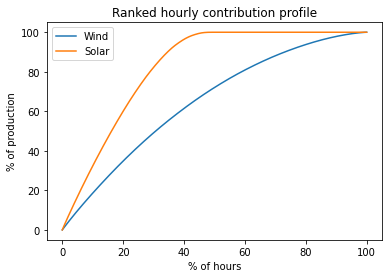
\includegraphics[width=1.0\textwidth]{renewable_production_hours_ranked}
	\caption[Percent of hours in a year contributing to a percent of the output, ranked by importance]{Percent of hours in a year contributing to a percent of the output, ranked by importance.}
	\labfig{renewable_production_hours_ranked}
\end{figure}

The \vreffig{renewable_production_hours_ranked} may be a bit difficult to read, so let me spend some time explaining what went on here. In order to generate this plot, I used one year of hourly power output for both wind and solar power. The solar data was simulated over Texas using synthetic solar photovoltaic from NREL. The wind data was downloaded from the ERCOT website, the Texan grid operator. This data consequently approximates potential redistribution of power generation between different part of the state of Texas.

Knowing the power generated every hour of the year, I then ranked them from most productive to least productive. So, if you take the solar data for example, the "noons" of the year are first, and the nightly hours come later, not contributing any power to the production. From that, I then plotted where each hour falls in the year ranking against the percentage of production.

In other words, what this graph shows is that for solar power, once you reach the 40\% of the top contributing hours, you have generated all the yearly power. The remaining 60\% do not contribute power. This is logical, as it is night 50\% of the time and your panels are more efficient in direct sunlight than in the evening, when it gets hit only by diffuse sunlight.

Another way of interpreting this graph is that 80\% of solar power production is done in only 30\% of the time during the year, leaving you at risk of not meeting production demand the rest of the time because you can easily find period where multiple consecutive hours are in those 70\% remaining hours.

Wind is less predictable, but has more contributing hours during a year. You do not have a clear cycle like nights and days, and it varies a bit more regionally than the sun irradiance. 80\% of the production from wind power comes from 60\% of the time, leaving you at risk during 40\%. Using this data, what we can conclude as a first order approximation is that your needs, with solar, would be covered 30\% of the time, while they would be covered 60\% of the time for wind\sidenote[][-2mm]{A complex model can give better results there, by combining the solar or wind data with an estimation of the hourly load notably, at the risk of over-optimization leading to a less resilient grid and more frequent blackouts. Our approach is still a pretty good first order approximation of the scale we are talking about.}.

Consequently, we can say that in the most favorable situation, wind would cover for solar at night, and wind is low only during the day.

\begin{remark}
In that case, based on a reasonable 80\% of the total production being viable:

\begin{itemize}
\item It's sunny enough for 30\% of the time, and not windy enough for 40\% of the time
\item It's windy enough for 60\% of the time, and not sunny enough for 70\% of the time
\end{itemize}

So, on first order approximation, we can say that 10\% of the energy need cannot be met, even under the most ideal, fairy tale scenario.

\end{remark}

One can consider adding hydroelectricity or geothermal to the mix and think that this could meet 100\% of the demands and to not have a storage requirements\sidecite{hoste2009matching,brown2018synergies}. It has however been shown to be reliant on assumptions that are on the very optimistic side\sidecite{boretti2020cost,clack2017evaluation}, notably because of short term strong variability. A different way to look at it is that it may work for larger regions with strong interconnections and links, such as the European Union and the United States of America, and in a beautifully engineered infrastructure which would have to be flawless\sidenote[][*6]{From a purely geopolitical and national security perspective, it is not far-fetched to consider the impact on balance of power at small and abrupt time scale.}.

%In this section, we will consider the short term unpredictable variability of solar and wind, and consider that even only 10\% of the energy needs have to come from storage\sidenote[][*6]{Keep in mind that while this is theoretically possible, it is physically unlikely to be the case. That's the limitation with theoretical models, they tend to assume that everything works a bit too much as expected}.


\begin{remark}

In this renewable energy mix scenario, which does imply an important paradigm shift in society consumption and grid operation to add leniency, the amount of storage needed consequently is given by~\ref{energy_store}, $t$ varying between 1 and 7 days and becomes:

\begin{equation}\label{energy_store}
E_s = f_s * t * \frac{E_a}{8760}
\end{equation}

Here, we assume, as seen previously, that an optimist assumption for the fraction of energy to store is $f_s = 10\%$.


\end{remark}


\section{Scenarios S3}

The S3 scenarios are made up of only one scenario, a 100\% nuclear grid. In order to get to this, we will first get rid of all the existing installed capacity, with the associated dismantling costs, and rebuild everything from scratch to cover the entirety of a country electricity needs.

Nuclear has shown that it can follow loads on short time scale. While some may disagree that a 100\% nuclear could function efficiently due to this issue, it is still a reasonable assumption to make.


\begin{kaobox}[frametitle=S3 scenarios]
\begin{itemize}
	\item \textbf{S3a:} 100\% Nuclear
\end{itemize}
\end{kaobox}


\section{Scenarios S4}

The nuclear and renewable mix is a scenario in which a given share of the energy production is driven by nuclear energy, while the rest is produced by renewables.

This presents, as will be demonstrated later on, a clear advantages in that it does not require large, grid-scale storage capabilities. It can answer to multiple concerns about all the scenarios S1, S2, and S3.

We vary the share of nuclear versus renewable energies to show the impact of a nuclear-heavy energy production as well as a renewable heavy production.


\begin{kaobox}[frametitle=S4 scenarios]
\begin{itemize}
	\item \textbf{S4a:} 50\% Nuclear, 50\% Renewables (30\% Wind onshore, 10\% Wind offshore and 60\% Solar)
	\item \textbf{S4b:} 50\% Nuclear, 50\% Renewables (40\% Wind onshore, 20\% Wind offshore and 40\% Solar)
	\item \textbf{S4c:} 25\% Nuclear, 75\% Renewables (30\% Wind onshore, 10\% Wind offshore and 60\% Solar)
	\item \textbf{S4d:} 25\% Nuclear, 75\% Renewables (40\% Wind onshore, 20\% Wind offshore and 40\% Solar)
	\item \textbf{S4e:} 75\% Nuclear, 25\% Renewables (30\% Wind onshore, 10\% Wind offshore and 60\% Solar)
	\item \textbf{S4f:} 75\% Nuclear, 25\% Renewables (40\% Wind onshore, 20\% Wind offshore and 40\% Solar)
\end{itemize}
\end{kaobox}





\section{The Digest}


\begin{kaoboxgreen}[frametitle=Main Takeaways]

\begin{itemize}
\item We define four main categories of scenarios, from all renewable to all nuclear, with some mixes.
\item Each categories is divided into a given number of scenarios where some parameters are modified.
\item Nineteen scenarios are computed to be representative of the potential options considered.
\end{itemize}
  
\end{kaoboxgreen}



















%Multiple scenarios will be tested from the two categories we defined.


%\begin{kaobox}[frametitle=Scenarios to consider]

%\begin{itemize}
%	\item S1: Onshore Wind -- Pumped Hydro Storage
%	\item S2: Onshore Wind -- Batteries
%\item S3: Offshore Wind -- Pumped Hydro Storage
%	\item S4: Offshore Wind -- Batteries
%	\item S5: Solar -- Pumped Hydro Storage
%	\item S6: Solar -- Batteries
%	\item S7: Nuclear
%	\item S8\footnote{We can vary the share of each technologies. By default, we use 30\% onshore wind, 10\% offshore wind,  60\% solar mix, and 50\% batteries, 50\% pumped storage}: Renewable Mix -- Storage Mix
%	\item S9\footnote{We can vary the share of each technologies. By default, we use 24\% wind onshore, 8\% wind offshore, 48\% solar, 20\% nuclear mix}: Nuclear -- Renewable Mix
%\end{itemize}

%Each of the scenarios will furthermore be tested for sensitivity by modifying parameters and looking at a range of future potentials, from pessimistic to optimistic depending on the energy source.

%\end{kaobox}